% !TeX spellcheck = pt_BR


\documentclass[12pt,a4paper,oneside,openany]{abntex2}

% PACOTES OBRIGATÓRIOS (Idioma e codificação)
\usepackage[utf8]{inputenc}
\usepackage[T1]{fontenc}
\usepackage[brazil]{babel}

% PACOTES PARA O TEXTO E CITAÇÕES
\usepackage{csquotes}      % Aspas inteligentes
\usepackage{graphicx}      % Inserir imagens
\usepackage{tabularx}
\usepackage{amssymb}

% PACOTES PARA A TABELA (NECESSÁRIOS)
\usepackage{array}         % Para \arraybackslash e \extrarowheight
\usepackage{booktabs}      % Para \toprule, \midrule, \bottomrule, \addlinespace
\usepackage[table]{xcolor} % Para \rowcolor
\usepackage{ragged2e}      % Alinhamento

% CONFIGURAÇÕES DE MARGEM E ESPAÇAMENTO
\setlrmarginsandblock{3cm}{2cm}{*}
\setulmarginsandblock{3cm}{2cm}{*}
\checkandfixthelayout
\OnehalfSpacing

\usepackage[
    backend=biber,
    style=abnt,
    natbib=true,
    hyperref=true
]{biblatex}
\addbibresource{6_referencias/referencias.bib}

\usepackage{hyperref}

\titulo{Análise de sinais Eletromiografia para uso de próteses}

\autor{Yuri Martins Alegre}
\data{2026}
\instituicao{Universidade Federal de Santa Catarina -- UFSC}
\newcommand{\centro}{Centro de Ciências, Tecnologias e Saúde -- CTS}
\newcommand{\curso}{Curso de Engenharia de Computação}
\newcommand{\cidade}{Araranguá}
\newcommand{\estado}{SC}
\newcommand{\ano}{2026}
\orientador{Prof. Rodrigo Pereira}
\coorientador{Prof. Lucas Bertinetti}

\renewcommand{\imprimircapa}{
    \begin{capa}
        \begin{center}
             \begin{figure}[h]
                 \center
             
\includegraphics[width=3.4cm]{Arquivos/Logo_Universidade.png}
             \end{figure}
             \vspace{1cm}
            
            \textsc{\imprimirinstituicao}\\
            \textsc{\centro}\\
            \textsc{\curso}\\
            
            \vspace{2.5cm}
            \imprimirautor
            
            \vspace{2.5cm}
            \textbf{\imprimirtitulo}
            
            \vfill
            
            \cidade/\estado\\
            \ano
        \end{center}
    \end{capa}
}

\renewcommand{\imprimirfolhaderosto}{
    \begin{folhaderosto}
                
        \begin{center}    
            \textsc{\imprimirtitulo}
        \end{center}
        
        \vspace{2cm}    
        
        \begin{center}
            \imprimirautor
        \end{center}
        
        \vspace{2.5cm}
        
        \hfill \parbox{8.5cm} {\noindent
            Relatório técnico de pré-projeto submetido à \imprimirinstituicao~como parte dos requisitos da disciplina de Projeto Integrador II, apresentando a proposta de desenvolvimento para o Trabalho de Conclusão de Curso do Bacharelado em Engenharia de Computação.            
            
            \vspace{0.5cm}
            Orientador: \imprimirorientador\\
            Coorientador: \imprimircoorientador
        }
        
        \vfill
        \vspace{2.0cm}
        
        \begin{center}
            \cidade/\estado\\
            \ano
        \end{center}
    \end{folhaderosto}
}

\begin{document}

\imprimircapa

\imprimirfolhaderosto

\pdfbookmark[0]{\contentsname}{toc}
\tableofcontents*
\cleardoublepage

\textual

% Certifique-se de que estes ./arquivos existam nos seus diretórios
\chapter{Introdução}

\section{Contexto e Motivação}

A perda de membros superiores representa um dos maiores desafios para a qualidade de vida de indivíduos acometidos por amputações traumáticas, congênitas ou decorrentes de doenças como diabetes e doenças vasculares periféricas. No Brasil, segundo dados do Sistema de Informações Hospitalares do SUS (SIH/SUS), foram realizados 49.165 procedimentos de amputação em 2011, sendo as causas externas (33,1\%), doenças infecciosas e parasitárias (17,9\%) e doenças do aparelho circulatório (16,1\%) as etiologias mais frequentes. Apesar de as amputações de membros inferiores corresponderem a aproximadamente 85\% de todos os casos, as amputações de membros superiores impõem impacto funcional severo, comprometendo diretamente a autonomia e a capacidade de realização das atividades de vida diária do indivíduo. \cite{Diretrizes}
\begin{figure}[htbp]
    \centering
    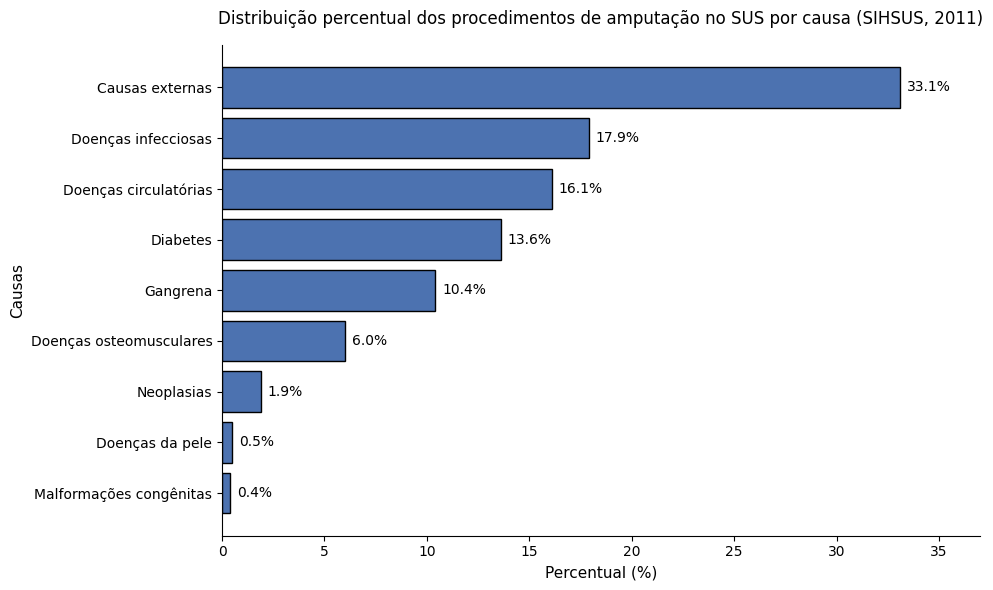
\includegraphics[width=0.8\textwidth]{1_introducao/assets/frequencia_amputacao.png}
    \caption{Distribuição percentual dos procedimentos de amputação no SUS por causa \cite{Diretrizes}.}
    \label{fig:amputacoes}
\end{figure}

Neste cenário, as próteses robóticas controladas por sinais biológicos emergem como uma alternativa promissora.
\section{Justificativa}

Apesar do crescente número de publicações na área de controle de próteses por eletromiografia de superfície (sEMG, do inglês \textit{Surface Electromyography}), ainda existe uma lacuna significativa entre os protótipos de laboratório e dispositivos funcionais, acessíveis e de fácil reprodução. A maioria dos sistemas disponíveis comercialmente apresenta custo elevado, o que restringe seu acesso. Além disso, soluções acadêmicas frequentemente utilizam hardware proprietário ou de difícil aquisição no contexto brasileiro.

Como proposta de desenvolvimento, será empregado microcontroladores COTS (componentes comerciais prontos para uso, do inglês \textit{Commercial Off-The-Shelf}) , amplificadores operacionais, eletrodos de sEMG, softwares de simulação, programação e estruturas mecânicas fabricadas por impressão 3D, aliados a técnicas modernas de aprendizado de máquina para classificação de gestos.


\section{Objetivo}

Como Objetivo Geral este trabalho proprõe desenvolver um sistema capaz de capturar sinais de sEMG, classificar movimentos da mão e do braço por meio de técnicas de aprendizado de máquina e reproduzi-los em uma prótese robotica. De formar mais específica, este trabalho proprõe:
\begin{itemize}
    \item Projetar, simular e implementar o circuito de aquisição e processamento do sinal;
    \item Desenvolver, testar e validar o firmware de aquisição no hardware transmissor;
    \item Construir e treinar um modelo de aprendizado de máquina para classificação de 5 a 8 gestos distintos;
    \item Desenvolver, testar e validar o firmware de controle no hardware receptor;
\end{itemize}

\section{Metodologia}

A metodologia adotada segue uma abordagem de desenvolvimento iterativo e incremental, organizada em cinco etapas principais. 

Na primeira etapa, realiza-se a revisão bibliográfica sobre processamento de sinais sEMG, técnicas de aprendizado de máquina aplicadas à classificação de gestos e sistemas embarcados para controle de próteses.

Na segunda etapa, projeta-se e implementa-se o hardware de condicionamento de sinal, composto por filtros passa-altas, passa-baixas e rejeita-faixa (notch), amplificadores de instrumentação e circuitos de retificação e envoltória. Os sinais condicionados são digitalizados pelo conversor analógico-digital do hardware transmissor e enviados ao hardware receptor.

Na terceira etapa, utiliza-se o dataset público NinaPro \cite{Ninapro} DB2 (Non-Invasive Adaptive Prosthetics Database 2) como base inicial para o desenvolvimento e validação do modelo de aprendizado de máquina, antes da coleta de dados com voluntários. O NinaPro DB2 contém registros de sEMG de 40 sujeitos íntegros realizando 49 movimentos de mão, capturados com 12 eletrodos Delsys Trigno a uma taxa de amostragem de 2 kHz, com 6 repetições de cada movimento por sujeito \cite{Atzori2014Electromyography}. A utilização dessa base pública permite o desenvolvimento e a avaliação dos algoritmos de classificação em um conjunto de dados amplo e validado pela comunidade científica, reduzindo o risco de overfitting e acelerando o ciclo de desenvolvimento. Previamente à etapa de coleta com voluntários, o protocolo experimental será submetido à aprovação do Comitê de Ética em Pesquisa (CEP) por meio da Plataforma Brasil, e todos os participantes assinarão o Termo de Consentimento Livre e Esclarecido (TCLE). Após a validação do pipeline de processamento e classificação sobre o NinaPro DB2 e a obtenção das aprovações éticas necessárias, procede-se à coleta de dados sEMG de voluntários saudáveis realizando os 5 a 8 gestos-alvo selecionados para o sistema protético, visando à adaptação e ao ajuste fino do modelo ao hardware desenvolvido.

\chapter{Fundamento Teórico}

\section{Eletromiografia de Superfície (sEMG)}

A eletromiografia consiste em uma técnica de registro da atividade elétrica produzida pelos músculos esqueléticos durante a contração. Quando um neurônio motor dispara, propaga-se ao longo das fibras musculares uma diferença de potencial denominada potencial de ação da unidade motora (PAUM). A eletromiografia de superfície (sEMG) capta a superposição temporal e espacial desses PAUMs por meio de eletrodos posicionados sobre a pele, de forma não invasiva, diferindo da eletromiografia intramuscular, que utiliza agulhas inseridas diretamente no tecido muscular.\cite{Costa}
\begin{figure}[htbp]
    \centering
    \caption{Ilustração do processo de aquisição de sinais sEMG}
    \label{fig:ilustracaosensor}
    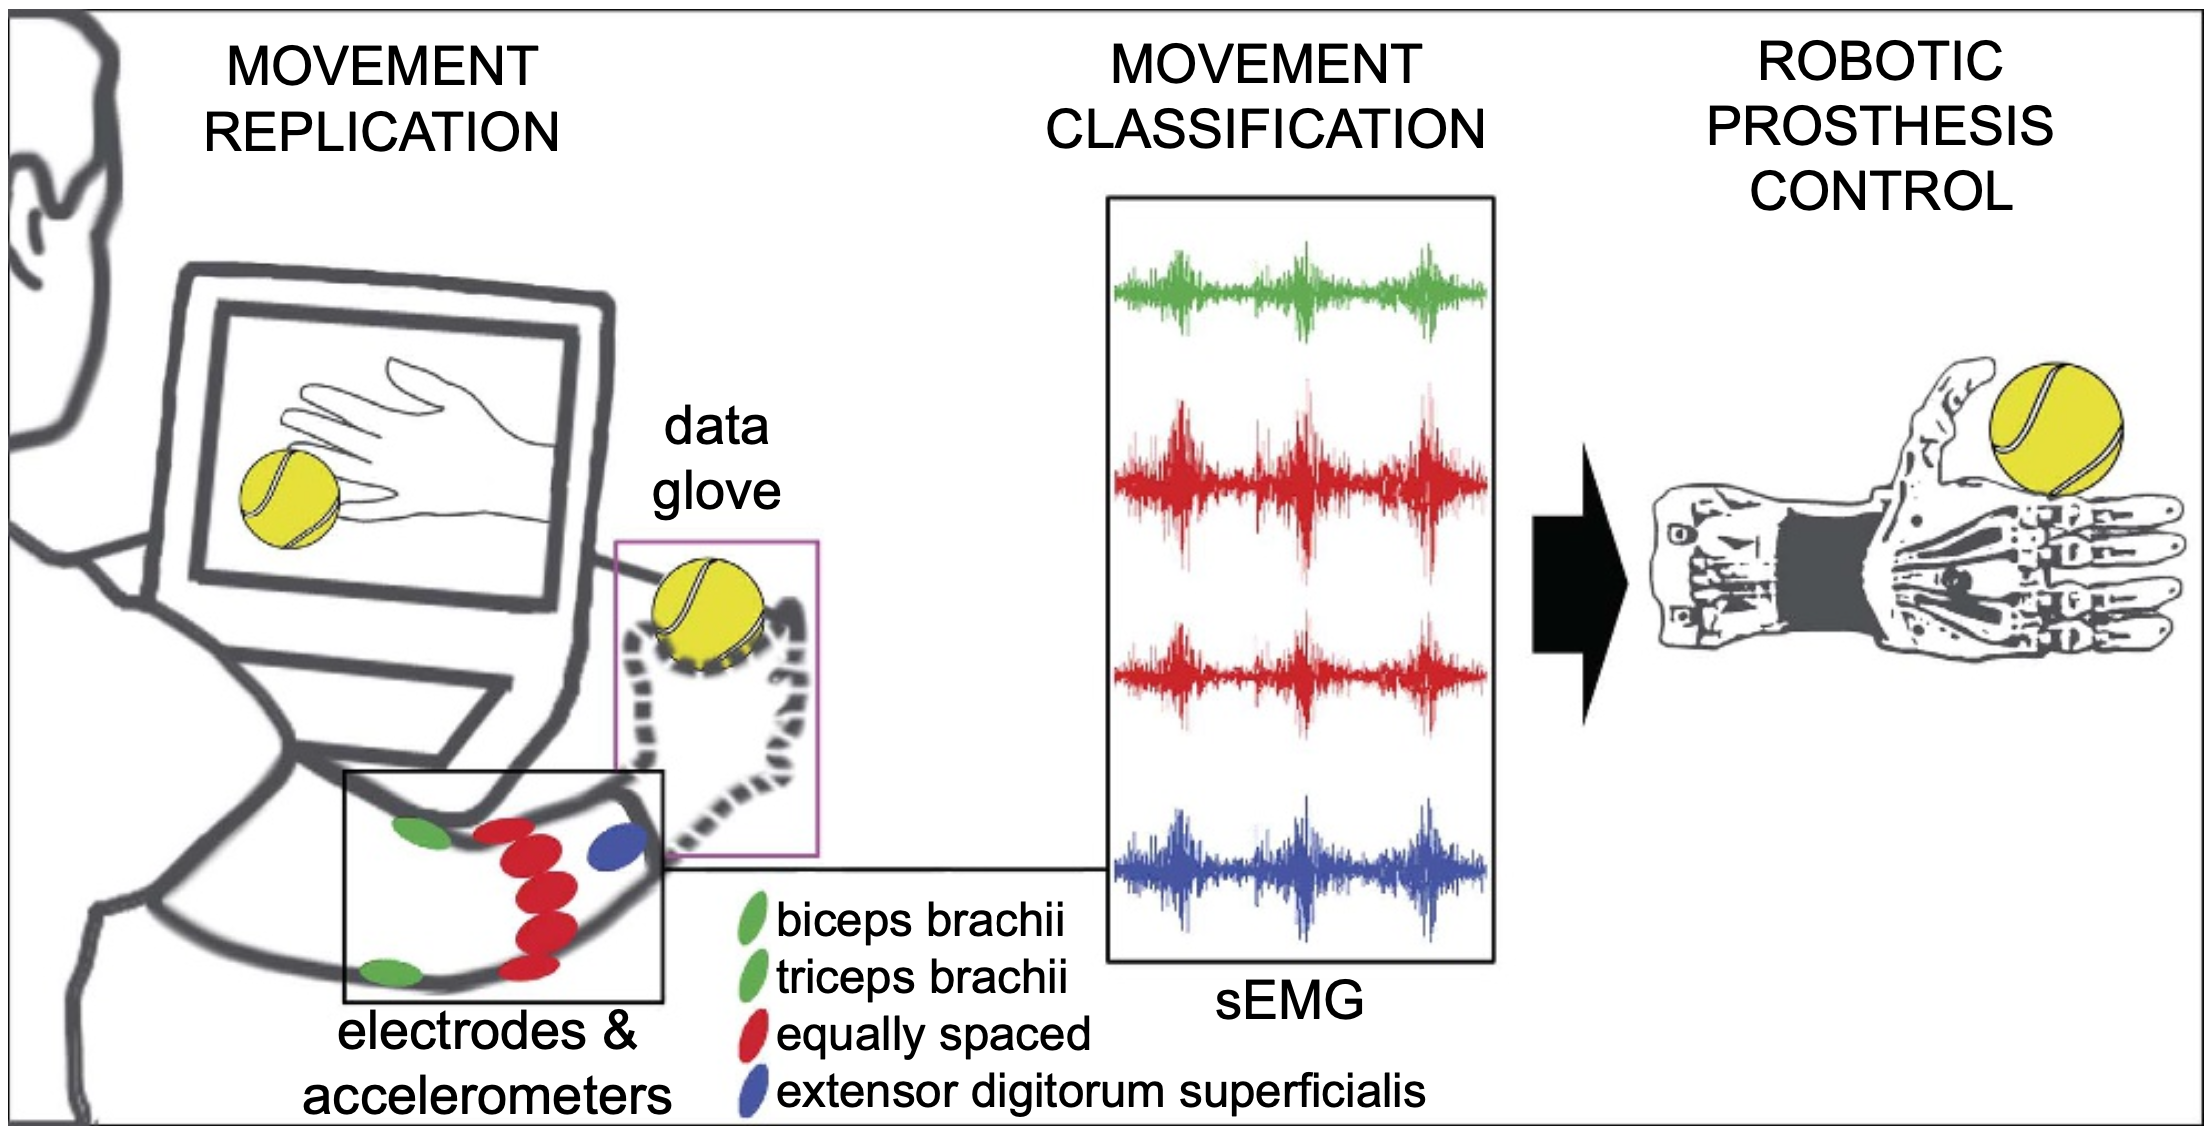
\includegraphics[width=0.8\textwidth]{2_fundamento_teorico/assets/SData_Protocol.png}
    \fonte{\cite{Ninapro}.}
\end{figure}

O sinal sEMG apresenta amplitude tipicamente entre 1 mV e 10 mV, frequências úteis na faixa de 20 Hz a 500 Hz, elevada sensibilidade a ruídos e forte dependência de fatores como posicionamento dos eletrodos, espessura do tecido subcutâneo, temperatura e fadiga muscular. Suas principais fontes de interferência incluem o ruído da rede elétrica (50/60 Hz), artefatos de movimento dos eletrodos, ruído térmico (Johnson), crosstalk de grupos musculares adjacentes e artefatos de movimento corporal.
Para minimizar essas interferências, é necessário um cuidadoso condicionamento do sinal, composto tipicamente por um amplificador de instrumentação (ganhos entre 100 e 1000), filtros passa-altas (corte em torno de 20 Hz para remoção de artefatos DC e de movimento), filtros passa-baixas (corte em 500 Hz), filtro notch (50 ou 60 Hz) e, opcionalmente, etapas de retificação e extração de envoltória para análise de amplitude.\cite{CLANCY20021}

\section{Aquisição de Dados}
O circuito de aquisição de sinais sEMG é projetado para amplificar e filtrar o sinal captado pelos eletrodos antes de sua digitalização. O amplificador de instrumentação, como o INA128 ou o AD8221, é responsável pela amplificação diferencial do sinal com alta rejeição ao modo comum (CMRR), fundamental para eliminar interferências eletromagnéticas presentes no ambiente clínico e laboratorial.

Após a amplificação, o sinal passa por uma cadeia de filtros analógicos: um filtro passa-altas de segunda ordem (tipicamente Butterworth) com frequência de corte de 20 Hz remove componentes DC e artefatos de baixa frequência; um filtro passa-baixas com corte em 500 Hz limita a banda de interesse; e um filtro notch em 60Hz (padrão brasileiro) atenuar a interferência da rede elétrica. O sinal condicionado é então amostrado pelo conversor analógico-digital (ADC) do microcontrolador com frequência de amostragem de pelo menos 1 kHz (conforme o critério de Nyquist para a faixa de interesse).

\begin{figure}[htbp]
    \centering
    \caption{Fluxograma das etapas de amplificação e filtragem do sinal sEMG}    
    \label{fig:fluxogramafiltros}
    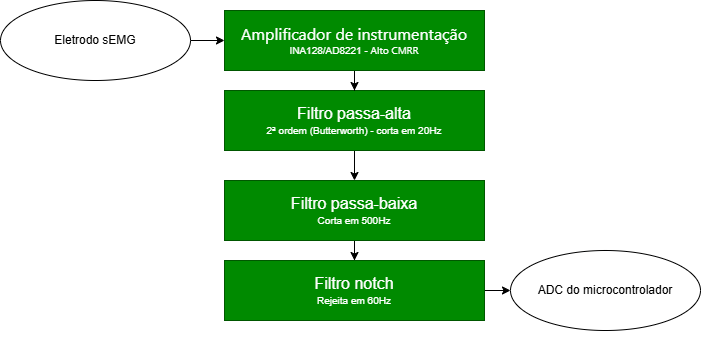
\includegraphics[width=0.8\textwidth]{2_fundamento_teorico/assets/FluxogramaFiltros.png}
    \fonte{Elaborado pelo autor (2026)}
\end{figure}
\section{Microcontrolador}

O ESP32 \cite{esp32_datasheet} é um microcontrolador de duplo núcleo (Xtensa LX6, 240 MHz) desenvolvido pela Espressif Systems, dotado de conectividade Wi-Fi 802.11 b/g/n e Bluetooth 4.2/BLE integrados, ADC de 12 bits com 18 canais, memória flash de 4 MB e suporte a protocolo SPI, I2C e UART. Sua ampla disponibilidade, baixo custo e capacidade de processamento em tempo real tornam adequado tanto para a aquisição e transmissão dos sinais sEMG (ESP32 transmissor) quanto para o processamento e controle da prótese (ESP32 receptor).
A comunicação entre os dois módulos ESP32 pode ser realizada via protocolo ESP-NOW, que oferece baixa latência, baixo consumo energético e conexão ponto a ponto sem necessidade de infraestrutura de rede, sendo ideal para aplicações em tempo real como o controle protético


\section{Extração de Características e Aprendizado de Máquina}
A classificação de gestos a partir de sinais sEMG requer a extração de características discriminativas que representem adequadamente os padrões musculares associados a cada movimento \cite{Castro}. No domínio do tempo, as características mais utilizadas incluem o valor RMS (Root Mean Square), o valor médio absoluto (MAV), a variância, a taxa de cruzamentos por zero (ZC) e o comprimento de forma de onda (WL). No domínio da frequência, a frequência mediana, a frequência média e a potência em sub-bandas específicas fornecem informações complementares sobre o recrutamento das unidades motoras.
Embora existam diversos algoritmos de classificação amplamente consolidados na literatura para sinais sEMG, como Máquinas de Vetores de Suporte (SVM), Redes Neurais Artificiais (RNA) do tipo MLP e modelos de Floresta Aleatória (Random Forest), a proposta deste trabalho consiste em realizar uma etapa prévia de filtragem dos sinais e, em seguida, utilizar Redes Neurais Convolucionais (CNNs), em consonância com a abordagem proposta em "Multiday EMG-Based Classification of Hand Motions with Deep Learning Techniques"  \cite{Rehman} . Essa estrutura apresenta a vantagem de remover ruídos e interferências na etapa de pré-processamento, permitindo que a CNN realize a extração automática de características diretamente das ondas filtradas.

\section{Trabalhos relacionados}

A qualidade dos sinais eletromiográficos de superfície (sEMG) é fator determinante para o sucesso de sistemas de reconhecimento de gestos e controle de próteses. A literatura recente tem concentrado esforços tanto no \textit{hardware} de aquisição, multiplicando canais e integrando filtros embarcados, quanto no pré‑processamento digital, etapa essencial para reduzir ruídos e artefatos antes da classificação.
A Tabela~\ref{tab:aquisicao_semg} sumariza os principais trabalhos que abordam a aquisição e a filtragem de sinais sEMG, evidenciando as soluções adotadas em diferentes épocas e contextos.

\begin{table}[htpb]
    \centering
    \small
    \setlength{\extrarowheight}{3pt}
    \caption{Trabalhos relacionados focados na aquisição e filtragem de sinais sEMG.}
    \label{tab:aquisicao_semg}
    \begin{tabularx}{\textwidth}{@{} 
        >{\RaggedRight\arraybackslash}X 
        >{\RaggedRight\arraybackslash}X 
        >{\RaggedRight\arraybackslash}X 
        @{}}
        \toprule
        \rowcolor{gray!20} \textbf{Título do Artigo (Ano)} & \textbf{Sensor (Dispositivo, Quantidade e Canais)} & \textbf{Filtros Usados (Pré-processamento)} \\
        \midrule
        \textit{Processing and Analysis of EMG Signals from MYO Armband for Upper-Limb Prosthesis Control} \cite{ProcessingAndAnalysisOfEMGSignalsFromMYO} & 1 dispositivo (Myo Armband). 8 canais de eletrodos a seco posicionados ao redor do antebraço. & Filtro Passa-banda de 20--90 Hz e Filtro \textit{Notch} de 50 Hz. Retificação e suavização (RMS). \\
        \addlinespace
        \textit{High-Performance Surface Electromyography Armband Design for Gesture Recognition} \cite{Zhang2023-gn} & 1 bracelete customizado ($\alpha$ Armband). 16 canais com conversores ADC de 16-bit. & Largura de banda ajustável de 0.1 Hz a 20 kHz. Filtragem no hardware para capturar altas frequências. \\
        \addlinespace
        \textit{Medium density EMG armband for gesture recognition} \cite{Aghchehli2025-te} & 1 bracelete de “Média Densidade” customizado. 21 canais usando eletrodos digitais de contato por mola. & Filtro de Interferência Eletromagnética (EMI) integrado no hardware. IA minimiza necessidade de filtros digitais. \\
        \addlinespace
        \textit{Machine Learning Approaches for EMG Signal Classification to Predict Hand Gesture} \cite{Rendon_Caballero2026-ar} & Eletrodos de superfície padrão. Comparação entre matrizes de 10, 7 e 4 canais. & Filtro \textit{Notch} de 50 Hz e Filtro Passa-banda de 50--500 Hz. Segmentação em janelas de tempo curtas. \\
        \addlinespace
        \textit{putEMG—A Surface Electromyography Hand Gesture Recognition Dataset}\cite{Kaczmarek2019-mw}  & Matriz de eletrodos sEMG no antebraço coletando dados em altíssima densidade via 24 canais. & Filtros digitais passa-baixo e passa-alto nos dados brutos para estabelecer o \textit{baseline} de classificação. \\
        \bottomrule
    \end{tabularx}
\end{table}

A análise conjunta dos trabalhos revela três tendências claras:
\begin{enumerate}
    \item \textbf{Densificação dos canais}: Os sistemas evoluíram de 8 canais (Myo Armband) para arranjos com 21 ou 24 canais, buscando maior resolução espacial do sinal.
    \item \textbf{Pré‑processamento \textit{on‑chip}}: A filtragem analógica ou digital embarcada (EMI, banda ajustável) vem ganhando espaço, reduzindo a carga sobre o software de classificação.
    \item \textbf{Par mínimo de filtros digitais}: A combinação de um filtro passa‑banda (tipicamente 20–500 Hz) com um filtro \textit{notch} em 50 Hz (ou 60 Hz) persiste como prática padrão, mesmo quando métodos de aprendizado de máquina são empregados na etapa seguinte.
\end{enumerate}
Essas constatações orientam a escolha do \textit{hardware} e da cadeia de filtros adotados no presente trabalho, que busca equilibrar densidade de canais, qualidade do sinal e complexidade computacional.
\chapter{Proposta de Desenvolvimento}

\section{Descrição Geral do Sistema}
O sistema proposto consiste em uma prótese robótica de mão e braço controlada por sinais de eletromiografia de superfície, com comunicação sem fio entre dois módulos ESP32. A Figura \ref{fig:Fluxograma} ilustra a arquitetura geral do sistema, composta pelos seguintes subsistemas:
\begin{itemize}
    \item Módulo de aquisição: eletrodos sEMG posicionados sobre os músculos do antebraço do usuário, conectados a um circuito de condicionamento de sinal (amplificação e filtragem), cuja saída é digitalizada pelo ESP32 transmissor;
    \item Módulo de processamento e comunicação: o ESP32 transmissor realiza a segmentação das janelas de sinal, a extração de características e a classificação do gesto por meio do modelo de aprendizado de máquina embarcado, transmitindo o rótulo do gesto reconhecido via ESP-NOW ao ESP32 receptor;
    \item Módulo de controle da prótese: o ESP32 receptor recebe o comando de gesto e aciona os servomotores por sinais PWM, reproduzindo o movimento correspondente.   

\end{itemize}
 \begin{figure}[htbp]
    \centering
    \caption{Fluxograma do funcionamento geral}
    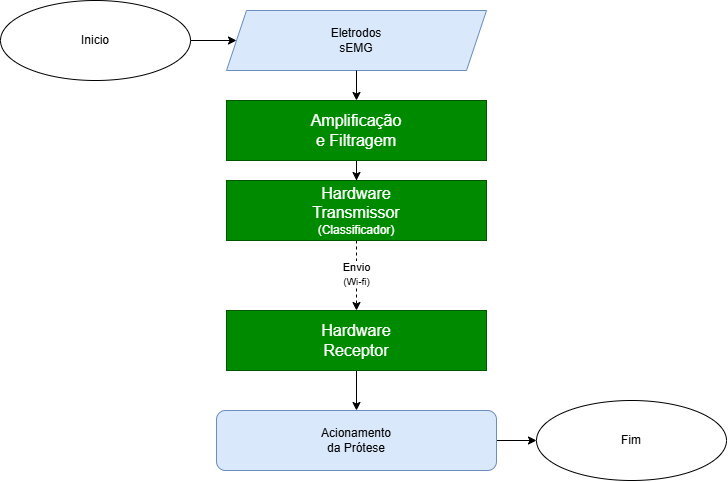
\includegraphics[width=1\textwidth]{3_proposta_desenvolvimento/assets/FluxogramaGeralHorizontal.png}
    \fonte{Elaborado pelo autor (2026)}
    \label{fig:Fluxograma}
\end{figure}
\section{Hardware de Condicionamento de Sinal}
O circuito de condicionamento será projetado para operar com dois canais  diferenciais (configuração bipolar) \cite{Krasoulis2020Multi}, utilizando o amplificador. O projeto incluirá: filtro passa-altas ativo de 2ª ordem para remoção de componentes DC; filtro notch passivo ou ativo em 60 Hz; filtro passa-baixas ativo de 2ª ordem ; estágio de ganho ajustável; e circuito de polarização para adequação do nível DC ao range do ADC do hadware transmissor (0–3,3 V). 

\section{Firmware hardware Transmissor}
O firmware do hardware transmissor será responsável pela amostragem dos canais ADC a 1 kHz, pela segmentação do sinal em janelas deslizantes de 200 ms com sobreposição de 50\%, pela extração das características selecionadas e pela execução do modelo de classificação em tempo real. O gesto classificado será transmitido via protocolo ESP-NOW ao receptor.

\section{Firmware hardware Receptor e Controle da Prótese}
O receptor receberá os comandos de gesto e acionará os servomotores por meio de sinais PWM, de acordo com uma tabela de mapeamento gesto-posição. O sistema prevê o controle de até 5 servomotores, um por dedo, além de um servo adicional para controle de rotação do punho. O firmware implementará uma máquina de estados para transições suaves entre gestos, evitando movimentos bruscos que possam danificar a estrutura mecânica.


%\section{Estrutura Mecânica da Prótese}


\section{Coleta de Dados e Treinamento do Modelo}
A coleta de dados sEMG será realizada com voluntários saudáveis realizando os 5 a 8 gestos-alvo, como: repouso, fechar mão (preensão de força), abertura total da mão, pinça lateral, pinça tripla digital, punho fechado, extensão de polegar e pronação/supinação\cite{Rehman}. Serão coletadas pelo menos 30 repetições por gesto por voluntário, com segmentação em janelas de 200 ms.

\chapter{Cronograma}
O cronograma a seguir apresenta uma proposta de distribuição das atividades ao longo das disciplinas TCC1 e TCC2, considerando um semestre letivo de aproximadamente 6 meses cada. A divisão exata entre as etapas será definida em conjunto com o orientador no início de cada disciplina. 
\begin{table}[htbp]
\centering
\resizebox{\textwidth}{!}{%
\begin{tabular}{|p{6.5cm}|*{12}{>{\centering\arraybackslash}p{0.45cm}|}}
\hline
\textbf{Atividade} & \textbf{1} & \textbf{2} & \textbf{3} & \textbf{4} & \textbf{5} & \textbf{6} & \textbf{7} & \textbf{8} & \textbf{9} & \textbf{10} & \textbf{11} & \textbf{12} \\ \hline
Revisão bibliográfica e fundamentação teórica & \checkmark & \checkmark & & & & & & & & & \checkmark&\checkmark \\ \hline
Modelagem e simulação do sinal sEMG em software & & \checkmark & \checkmark & & & & & & & & & \\ \hline
Projeto e aquisição do circuito de condicionamento de sinal & & \checkmark & \checkmark & & & & & & & & & \\ \hline
Coleta e pré-processamento de dados sEMG & & & \checkmark & \checkmark & & & & & & & & \\ \hline
Redação do TCC1 e apresentação parcial & & & & \checkmark & \checkmark & \checkmark & & & & & & \\ \hline
Finalização da coleta e integração hardware & & & & & & & \checkmark & \checkmark & & & & \\ \hline
Desenvolvimento do firmware (comunicação e leitura de sinais) & & & & & & & & \checkmark & \checkmark & & & \\ \hline
Projeto mecânico (CAD) & & & & & & & & & \checkmark & \checkmark & & \\ \hline
Integração completa (HW + FW) e ajustes & & & & & & & & & & \checkmark & \checkmark & \\ \hline
Validação de desempenho, testes finais e correções & & & & & & & & & & & \checkmark & \checkmark \\ \hline
Redação final e apresentação do TCC2 & & & & & & & & & & & & \checkmark \\ \hline
\end{tabular}%
}
\caption{Cronograma distribuído em 12 meses (TCC1: M1 a M6; TCC2: M7 a M12).}
\end{table}
\chapter{Considerações Finais}

Este relatório técnico apresentou a proposta estruturada para o desenvolvimento de um sistema de controle de próteses robóticas de membro superior, fundamentado na aquisição, processamento e classificação de sinais de eletromiografia de superfície (sEMG). A motivação central do projeto apoia-se na necessidade de desenvolver tecnologias assistivas funcionais, acessíveis e reprodutíveis., buscando mitigar a atual lacuna entre protótipos acadêmicos isolados e produtos comerciais de alto custo.

A arquitetura do sistema proposta demonstra viabilidade técnica ao integrar hardwares de baixo custo e alta capacidade de processamento, como os microcontroladores ESP32, a um circuito robusto de condicionamento analógico do sinal biológico. Além disso, a adoção de Redes Neurais Convolucionais (CNNs) para a extração automática de características e classificação dos gestos representa uma abordagem moderna e promissora. A estratégia metodológica de utilizar inicialmente a base de dados pública e validada NinaPro DB2 garante um ambiente seguro para o treinamento e ajuste fino dos modelos de aprendizado de máquina, reduzindo riscos de overfitting antes da etapa prática de coleta de dados com voluntários.

Por fim, o embasamento teórico consolidado e a metodologia aqui estabelecida fornecem as bases necessárias para a execução do projeto. O cronograma estipulado delineia claramente o roteiro de atividades para os próximos doze meses, englobando as disciplinas de Trabalho de Conclusão de Curso I e II. A expectativa é que, ao término deste ciclo, seja entregue um protótipo mecatrônico funcional e validado, contribuindo de forma significativa para as áreas de sistemas embarcados, inteligência artificial aplicada e engenharia de reabilitação.

\chapter*{Referências}
\addcontentsline{toc}{chapter}{Referências}
\printbibliography[heading=none]

\end{document}